\begin{center}
	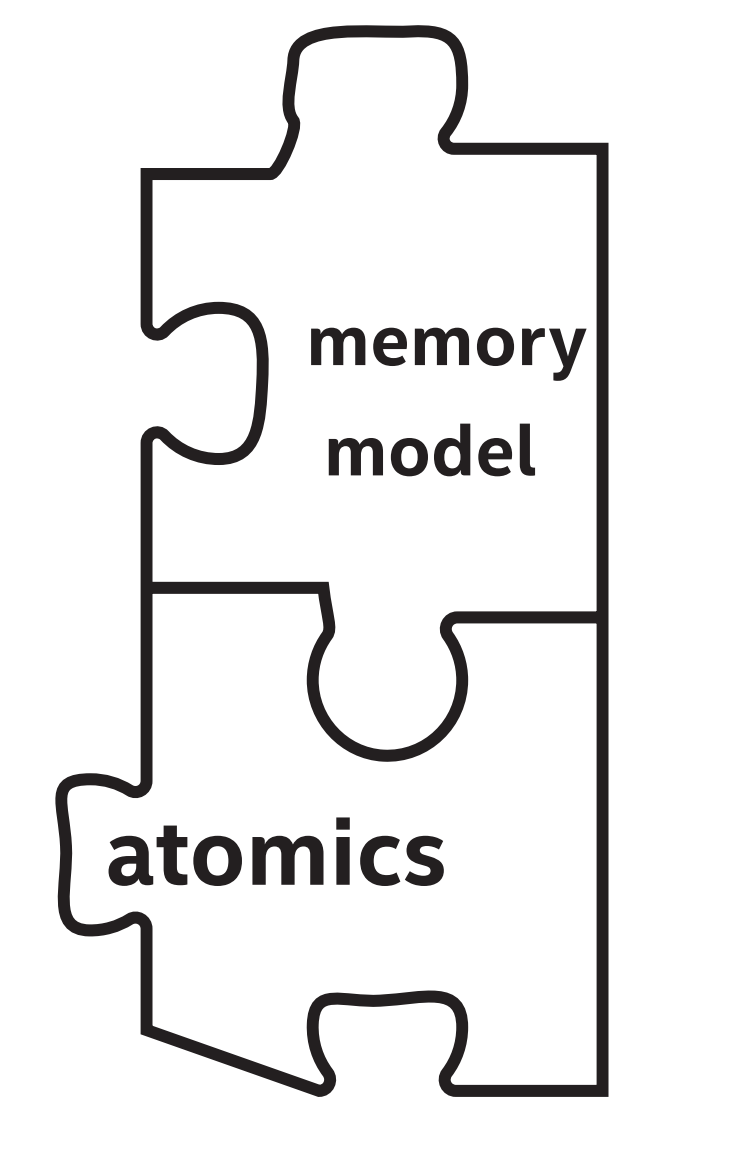
\includegraphics[width=0.5\textwidth]{content/chapter-19/images/1}
\end{center}

如果我们想成为优秀的并行开发者,内存一致性需要进行了解。它是我们拼图的关键部分,帮助我们确保数据在需要时就在需要的地方。这一章阐明了我们需要掌握的关键问题,以确保我们的程序正常运行。本主题不是SYCL或DPC++特有。\par

对于内存进行并发更新来说,对编程语言的内存(一致性)模型有基本的了解是必要的(这些更新是来自同一个内核中的多个工作项,多个设备,或者两者都是)。无论内存是如何分配的,这都是正确的,无论选择使用缓冲区还是USM分配,本章的内容对我们来说都很重要。\par

在前面的章节中,我们重点讨论了简单内核的开发,在这些内核中,实例要么操作完全独立的数据,要么使用结构化通信模式共享数据,这些模式可以使用语言和/或库直接表示。当要编写更复杂和更现实的内核时,可能会遇到这样的情况:程序实例可能需要以更不结构化的方式进行通信——要完成可移植的高效程序,理解内存模型如何与DPC++语言特性和硬件功能相关联是正确设计的必要前提。\par

标准C++的内存一致性模型足以编写完全在主机设备上执行的应用程序,但DPC++对其进行了修改,以解决在编写异构系统时可能出现的复杂性,以及在讨论程序实例时不能清晰地映射到C++线程概念时可能出现的复杂性。因此,我们需要了解\par

\begin{itemize}
	\item 系统中设备可以访问哪些类型的内存分配:使用缓冲区和USM。
	\item 内核执行期间防止不安全的并发内存访问(数据竞争):使用栅栏和原子操作。
	\item 启用执行相同内核的程序实例之间的安全通信,以及不同设备之间的安全通信:使用barrier、fence、atomics、memory order和memory scope。
	\item 防止与期望不兼容的优化:使用barriers, fences, atomics, memory orders和memory scope。
	\item 启用依赖于开发者的优化: 使用memory orders和memory scope。
\end{itemize}

内存模型是一个复杂的主题,可以根据兴趣进行了解——处理器架构师关心的是让处理器和加速器尽可能高效地执行代码!本章中,我们已经努力打破了这种复杂性,并强调了关键的概念和语言特性。本章开启了一条道路,不仅了解内存模型的内部和外部,并且享受并行编程。如果这里的描述和示例代码存在问题,强烈推荐访问本章末尾列出的网站或参考C++、SYCL和DPC++语言规范。\par














































